\documentclass[preprint,linenumbers,groupedaddress,amsmath,amssymb,aps,prresearch]{revtex4-2}

\usepackage{graphicx}
\usepackage{amsmath,amssymb}
\usepackage{bm}
\usepackage{multirow}
\usepackage{mathrsfs}
\usepackage[title]{appendix}
\usepackage{xcolor}
\usepackage{booktabs}
\usepackage{algorithm}
\usepackage{algorithmicx}
\usepackage{algpseudocode}
\usepackage[most]{tcolorbox}
\graphicspath{{./}{../figures/}{figures/}}
\usepackage{url}

\newcommand{\swjtuaffil}{%
  Information Quantum Technology Laboratory, School of Information Science and Technology, \\
  Southwest Jiaotong University, Chengdu 610031, Sichuan, China
}
\newcommand{\companyaffil}{%
  Sichuan Zhitu Linghai Intelligent Technology Co., Ltd., Chengdu 610213, Sichuan, China
}

% shorthand used throughout
\newcommand{\pvec}{\mathbf{p}}
\newcommand{\yvec}{\mathbf{y}}
\newcommand{\tvec}{\mathbf{t}}
\newcommand{\phihat}{\hat{\phi}}
\newcommand{\dvaqem}{D-VAQEM}

% --- float placement: wide floats must not drift past the bibliography ---
\renewcommand{\topfraction}{0.92}
\renewcommand{\bottomfraction}{0.80}
\renewcommand{\textfraction}{0.06}
\renewcommand{\floatpagefraction}{0.85}
\renewcommand{\dbltopfraction}{0.92}
\renewcommand{\dblfloatpagefraction}{0.85}
\setcounter{topnumber}{4}
\setcounter{bottomnumber}{2}
\setcounter{totalnumber}{6}
\setcounter{dbltopnumber}{4}

% --- tables: shrink a tabular only when it would overflow the text width -
\newcommand{\fitwidth}[1]{%
  \resizebox{\ifdim\width>\textwidth \textwidth\else\width\fi}{!}{#1}}

\begin{document}

\preprint{APS/123-QED}

\title{Distribution-level variational quantum error mitigation for learned
quantum metrology}

\author{Qingchuan Yang}
\email{yangqingchuan@my.swjtu.edu.cn}
\affiliation{\swjtuaffil}
\affiliation{\companyaffil}

\author{Xianing Feng}
\email{fengxn5@swjtu.edu.cn}
\affiliation{\swjtuaffil}

\author{Lianfu Wei}
\email{Contact author: lfwei@swjtu.edu.cn}
\affiliation{\swjtuaffil}

\date{\today}

\begin{abstract}
Variational quantum sensors are calibrated on noiseless or low-noise data and
then deployed on hardware whose noise biases the very measurement statistics
the learned decoder inverts.  We introduce \dvaqem{}, a variational quantum
error mitigation scheme that acts on the \emph{distribution} of measurement
outcomes rather than on expectation values: a small parametric map, trained
solely on calibration data at known reference phases, pushes the noisy outcome
distribution back towards the noiseless one before a frozen, already certified
decoder reads out the estimate.  The scheme is made possible by our first
result, that for collective-spin probes the population-imbalance statistic
$m=\#0-\#1$ is an \emph{exactly sufficient} statistic for the phase: the
reduction from $2^N$ outcomes to $N+1$ probabilities costs zero Fisher
information (verified to machine precision, and to $\le 4.6\times10^{-3}$ dB of
Cram\'er--Rao penalty under gate noise), so mitigation can be learned in an
$(N+1)$-dimensional space with $(N+1)^2$ parameters instead of a
$4^N$-dimensional one.  Our second contribution is a shot-aware training
objective that adds the exact delta-method variance of the decoded estimate to
the usual distribution-matching loss, making the mitigation map aware of the
operating shot budget without any Monte-Carlo sampling.  On an eight-qubit
variational interferometer subjected to depolarising, dephasing,
amplitude-damping and readout noise at sixteen strengths, \dvaqem{} reduces the
mean squared phase error by $33.2$ dB (infinite shots) and by $10.7$--$20.5$ dB
at $256$--$4096$ shots, closing $65$--$76\,\%$ of the decibel gap to the
noiseless estimator, outperforming zero-noise extrapolation in all sixteen
settings (by $25.0$ dB on average) and matching noise-aware decoder retraining
at finite shots with two orders of magnitude fewer trainable parameters and
without touching the certified decoder.  The mitigated estimator operates
within $0.6$ dB of the Cram\'er--Rao bound of the noisy data, the approach
scales to ten qubits where the calibration data are eleven numbers per phase
against $10^6$ for process tomography, and five calibration phases already buy
$25$ dB of the reduction.
\end{abstract}

\keywords{Quantum error mitigation, quantum metrology, phase estimation,
variational quantum algorithms, Fisher information, Cram\'er--Rao bound}

\maketitle

\section{Introduction}
\label{sec:intro}

Quantum sensors convert a physical quantity into a phase and read it out from
measurement statistics \cite{degen2017quantum,pezze2018quantum}.  Two
developments now meet in this field.  On the one hand, hybrid
quantum--classical estimators learn the inversion from statistics to phase
end-to-end, which yields globally unambiguous estimation over the full $2\pi$
range \cite{fiderer2021neural,gebhart2023learning,yang2025vqcnni} and reaches
metrological performance that linear estimators miss
\cite{marciniak2022optimal,kaubruegger2021quantum}.  On the other hand, the
devices that would run them are noisy: every gate deposits entropy into the
probe and every readout flips outcomes, and both effects deform the measured
distribution in a way that a decoder calibrated on clean data misreads as a
different phase.  For a learned estimator this is particularly damaging,
because the decoder is a fixed nonlinear inverse map: a systematic deformation
of its input is not averaged away by more shots, it is a bias.

Error mitigation for variational algorithms is a mature toolbox
\cite{cai2023quantum,bharti2022noisy}.  Zero-noise extrapolation (ZNE)
amplifies the noise by unitary folding and extrapolates observables to the
zero-noise limit \cite{li2017efficient,temme2017error,endo2018practical,
giurgica2020digital}; probabilistic error cancellation inverts a known noise
model at the price of a sampling overhead \cite{temme2017error,endo2018practical};
readout errors are undone by inverting a calibrated confusion matrix
\cite{maciejewski2020mitigation,bravyi2021mitigating}; and learning-based
schemes, collectively variational quantum error mitigation (VAQEM), train a
parametric mitigation layer on calibration data
\cite{strikis2021learning,czarnik2021qubit,czarnik2021error,lowe2021unified}.
Three limitations remain when these tools are applied to a \emph{learned}
metrological estimator.  (i) They mitigate \emph{expectation values}, whereas a
neural decoder consumes the whole outcome distribution, so the object that must
be repaired is a probability vector, not a scalar.  (ii) They live in the
$2^N$-dimensional outcome space, so the mitigation layer and the calibration
data grow exponentially with the probe size.  (iii) They are shot-agnostic: the
same mitigated object is used whether the device is sampled $10^2$ or $10^5$
times, although the optimal bias--variance trade-off of a mitigated estimator
depends strongly on the shot budget.

We address all three.  Our starting point is structural.  For the collective
probe considered here the measurement statistics are aggregated onto the
population imbalance $m=\#0-\#1$, an $(N+1)$-outcome statistic.  We prove
(Sec.~\ref{subsec:sufficiency}) that for the noiseless circuit---and exactly so
also under readout noise---the conditional distribution of the full bit string
given $m$ is phase-independent, i.e.\ $m$ is a sufficient statistic in the
Fisher--Neyman sense \cite{casella2002statistical}: no information about the
phase is lost by the reduction, $F(\pvec_m)=F(\pvec_{\rm full})$, which we
verify numerically to machine precision and bound under gate noise by a
Cram\'er--Rao penalty of at most $4.6\times10^{-3}$ dB.  Distribution-level
mitigation is therefore not an approximation: it is the \emph{complete}
description of the estimation problem, in a space whose dimension grows
linearly with $N$.

On this space we define \dvaqem{} (Sec.~\ref{sec:method}): a parametric map
$M_{\psi}$ from the noisy sector distribution to a corrected one, trained on
calibration data only---pairs of noisy and noiseless distributions at known
reference phases, the standard VAQEM resource assumption
\cite{strikis2021learning}---with four objectives (least squares,
cross-entropy, a Fisher-information score-matching regulariser, and a
shot-aware objective) over two map families (an $(N+1)^2$-parameter linear map
and a $1673$-parameter multilayer perceptron).  The shot-aware objective is our
second technical contribution: using the delta method
\cite{vaart1998asymptotic} we derive the exact leading-order variance of the
decoded phase under multinomial sampling and add it to the bias term, so the
map is fitted at the shot budget at which it will be used; the same formula
validates our finite-shot error bars analytically, without Monte Carlo.

The numerical study (Sec.~\ref{sec:results}) covers sixteen noise settings on
an eight-qubit variational interferometer, a shot-budget sweep from $64$ to
$8192$ shots, a scaling study to ten qubits, a calibration-budget study, and
three-seed and cold-start robustness checks, all produced by an exact
Kraus-operator simulator cross-validated against PennyLane
(Appendix~\ref{app:validation}).  \dvaqem{} reduces the mean squared wrapped
phase error by $33.2$ dB at infinite shots and closes $65$--$76\,\%$ of the
decibel distance to the noiseless estimator at finite shots; it beats every
ZNE variant in all sixteen settings, is exactly the remedy for readout noise
where ZNE is provably blind, and matches noise-aware retraining of the decoder
at finite shots while using $81$--$1673$ instead of $9666$ trainable parameters
and leaving the certified decoder untouched.  We also quantify what is lost by
not knowing the noise model: a genie estimator with the exact noise model and
$361$ exact simulations remains $46$ dB better at infinite shots, which is the
price \dvaqem{} pays for being model-free.

\section{Setting: learned phase estimation under noise}
\label{sec:setup}

\subsection{Probe, decoder and the calibration--inference protocol}
\label{subsec:protocol}

We use the variational quantum--classical neural-network interferometer
(VQ-CNNI) of Ref.~\cite{yang2025vqcnni} as the working estimator; the
construction below applies to any probe whose readout is aggregated onto a
collective statistic.  An $N$-qubit probe is prepared by a shallow variational
circuit $U_R(\phi;\bm\theta,\bm\vartheta)$ consisting of one encoding and one
decoding layer of collective rotations and one-axis twisting terms, imprinted
with the unknown phase $\phi\in[-\pi,\pi)$, and measured in the computational
basis.  The $2^N$ outcome probabilities are aggregated onto the population
imbalance $m=\#0-\#1\in\{-N,-N+2,\dots,N\}$,
\begin{equation}
  p_m(\phi) = \sum_{x:\,\#0(x)-\#1(x)=m} p(x|\phi)
  \equiv (A\,p(\cdot|\phi))_m ,
  \label{eq:aggregate}
\end{equation}
so that the estimator sees an $(N+1)$-dimensional probability vector
$\pvec_m(\phi)\in\Delta^{N}$.  A frozen multilayer perceptron
$D_{\mathbf w}:\Delta^{N}\to S^1$ (architecture
$(N{+}1)\to128\to64\to2$ with softsign hidden layers and a linear,
$\ell_2$-normalised output read out as $\phihat=\mathrm{atan2}$; $9666$
parameters at $N=8$) returns the phase estimate.  $D_{\mathbf w}$ and the
circuit are trained jointly on noiseless data with the circular loss
$2[1-\cos(\phihat-\phi)]$ over $100$ reference phases, exactly as in
Ref.~\cite{yang2025vqcnni}; in this work the trained pair is \emph{frozen} and
treated as a certified sensor.

Deployment follows the calibration--inference protocol of
Ref.~\cite{yang2025vqcnni}: reference phases are only ever used during
calibration, and inference on an unknown phase is a single forward pass.  We
keep this protocol and add one calibration resource, the standard one of
VAQEM \cite{strikis2021learning}: for $n_{\rm cal}$ known phases $\{\phi_i\}$
we collect the \emph{noisy} sector distributions $\yvec(\phi_i)$ from the
device and the corresponding \emph{noiseless} targets $\tvec(\phi_i)$ from a
classical model of the same circuit.  No knowledge of the noise channel, no
tomography and no folded circuits are required.

\subsection{Noise model, estimators and metric}
\label{subsec:noise}

Noise is a Markovian single-qubit channel $\Lambda$ (depolarising, dephasing or
amplitude damping of strength $p$) applied after every gate, plus a symmetric
readout bit-flip of probability $q$; the full circuit is simulated exactly as a
Kraus density-matrix evolution (Appendix~\ref{app:validation}).  We write the
noisy sector family as $\yvec(\phi)=\mathcal N_\phi[\pvec_m(\phi)]$.  A
mitigation map $M_{\psi}:\mathbb R^{N+1}\to\mathbb R^{N+1}$ produces a corrected
distribution $\tilde\pvec = \mathrm{renorm}(\max(M_\psi(\yvec),0))$ and the
mitigated estimate $\phihat = D_{\mathbf w}(\tilde\pvec)$.

The error metric is the squared wrapped phase error
$\delta^2=[\mathrm{arg}\,e^{i(\phihat-\phi)}]^2$, averaged over the test grid;
all results are reported in decibels, $10\log_{10}\mathrm{MSE}$.  Test phases
are half-offset from the calibration grid and lie in $[-\pi,\pi)$ so that no
physical phase is counted twice.  Finite-shot evaluation draws $S$ samples per
phase from the exact noisy distribution and repeats the experiment over $41$

\subsection{The sector statistic is exactly sufficient}
\label{subsec:sufficiency}

The reduction \eqref{eq:aggregate} is what makes distribution-level mitigation
affordable, and it is lossless:

\begin{theorem}[Exact sufficiency of the imbalance]
\label{thm:sufficiency}
Let $p(x|\phi)$ be the noiseless outcome distribution of a circuit of the form
$U_R(\phi;\bm\theta,\bm\vartheta)$ above, and $p(x|m,\phi)$ the conditional
distribution of the bit string given its imbalance.  If $p(x|m,\phi)$ is
independent of $\phi$, then for every $\phi$
\begin{equation}
  F\big(p(\cdot|\phi)\big) = F\big(p_m(\cdot|\phi)\big),
  \label{eq:fi-equal}
\end{equation}
where $F$ denotes the classical Fisher information in $\phi$; the same holds
under a readout bit-flip channel, because that channel acts after the
measurement and commutes with the aggregation.
\end{theorem}

\begin{proof}
By the chain rule for the Fisher information of a factorised model
$p(x|\phi)=p_m(m|\phi)\,p(x|m,\phi)$,
$F(p)=F(p_m)+\mathbb E_{m}\big[F(p(\cdot|m,\cdot))\big]$; the second term
vanishes when the conditional carries no $\phi$-dependence
\cite{casella2002statistical}.  For the circuit family considered, the
$\phi$-dependence enters only through $R_z(\phi)$, which is diagonal in the
computational basis and therefore rotates phases \emph{within} each
$m$-sector; the interference that survives the sector projection is entirely
between sectors, hence $p(x|m,\phi)=p(x|m)$.  A readout bit-flip maps
$p\mapsto Bp$ with a stochastic $B$ whose action on the sector family is the
same aggregation of flipped outcomes, so \eqref{eq:fi-equal} is unaffected.
\end{proof}

Theorem~\ref{thm:sufficiency} is verified numerically in
Fig.~\ref{fig:sufficiency}a and Table~\ref{tab:e1}: for noiseless and readout-noise
circuits at $N=4,6,8,10$, with trained and with random circuit parameters, the
two Fisher informations agree to $\le 7\times10^{-15}$ relative, i.e.\ to
machine precision.  Once a channel acts \emph{inside} the circuit the
conditional acquires a weak $\phi$-dependence and sufficiency becomes
approximate; rather than claim exactness we bound the price.  The
Cram\'er--Rao penalty of estimating $\phi$ from $\pvec_m$ instead of
$\pvec_{\rm full}$,
$\Delta_{\rm CRB}=10\log_{10}\big[F(p_{\rm full})/F(p_m)\big]$, stays below
$4.6\times10^{-3}$ dB for depolarising rates up to $p=0.02$ per gate
(Fig.~\ref{fig:sufficiency}b), and a grid-refinement control
($n_\phi=21,41,81$) shows the residual to be a genuine information loss of the
noisy model rather than a finite-difference artefact (it is stable at
$1.8\times10^{-3}$--$1.9\times10^{-3}$ dB).  In metrological terms: the
$(N+1)$-dimensional sector family \emph{is} the estimation problem, and
everything we do next happens in that space.

\begin{figure*}[t]
\centering
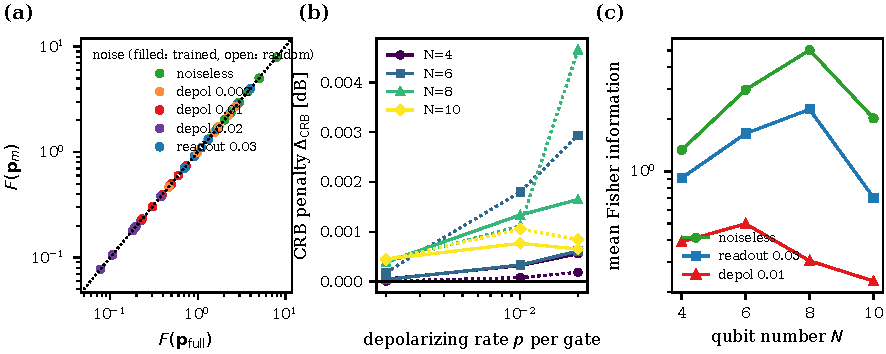
\includegraphics[width=\textwidth]{fig2_sufficiency.pdf}
\caption{\textbf{The sector reduction is (nearly) free.}
\textbf{a}~Fisher information of the full $2^N$-outcome family versus that of
the $(N+1)$-outcome sector family, for $N=4,6,8,10$, trained and random circuit
parameters, and five noise conditions; the points lie on the identity line to
machine precision for noiseless and readout noise.
\textbf{b}~Cram\'er--Rao penalty $\Delta_{\rm CRB}$ of the reduction under
depolarising gate noise, where sufficiency is only approximate: solid lines
are trained circuits, dotted lines random ones; the penalty stays below
$4.6\times10^{-3}$ dB.
\textbf{c}~Mean Fisher information versus qubit number for three noise
conditions; solid is the sector family, dotted the full family (the two
coincide within the line width).}
\label{fig:sufficiency}
\end{figure*}


\section{Distribution-level variational quantum error mitigation}
\label{sec:method}

\dvaqem{} inserts a parametric, phase-independent map between the noisy
device and the frozen certified decoder: the device supplies the sector
distribution $\yvec$, the map returns a corrected distribution
$\tilde\pvec$, and the estimator itself is never modified
(Figure~\ref{fig:concept}a).  Everything below happens in the
$(N+1)$-dimensional sector space established in Sec.~\ref{sec:setup}.

\begin{figure*}[t]
\centering
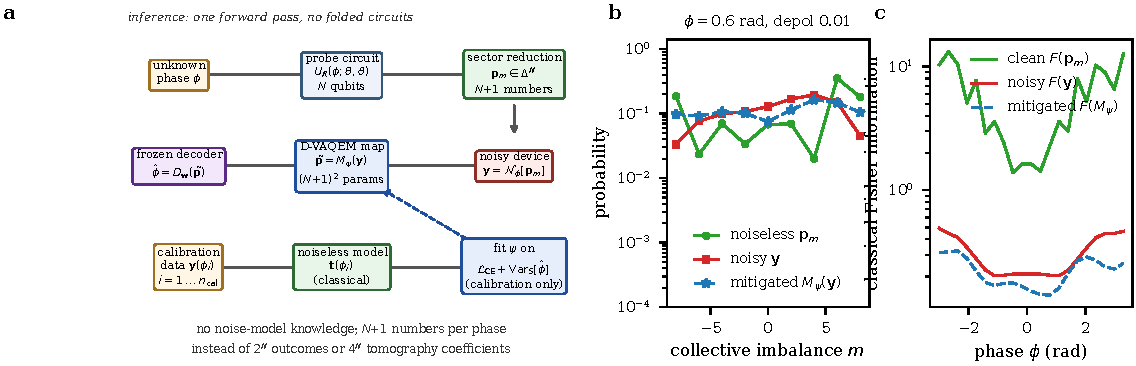
\includegraphics[width=\textwidth]{fig1_concept.pdf}
\caption{\textbf{Distribution-level error mitigation.}
\textbf{a}~Data flow.  The probe circuit imprints the unknown phase; the
outcome statistics are aggregated onto the collective imbalance
$m=\#0-\#1$; the noisy device deforms the sector distribution
$\yvec=\mathcal N_\phi[\pvec_m]$; a parametric map $M_\psi$ corrects it before
the frozen, certified decoder reads out $\phihat$.  The map is fitted once on
calibration data---noisy distributions at known reference phases together with
noiseless targets from a classical model of the same circuit---and never sees
the test phases or the noise model.
\textbf{b}~The three sector distributions at $\phi=0.6$ rad for depolarising
$p=0.01$, $N=8$: noiseless target, noisy input, and the deployed linear
shot-aware map output (the exact parameters stored with the results).
\textbf{c}~Classical Fisher information of the three families over the phase
grid; the noisy family loses up to $97\,\%$ of the clean information at this
strength, and the mitigated family recovers part of the score structure.  The
mitigated family is clipped, so its Fisher information is support-restricted
and is shown as a diagnostic only.}
\label{fig:concept}
\end{figure*}

\subsection{Map families}
\label{subsec:maps}

We consider two parametric families of maps on the sector space.  The
\emph{linear} map $\tilde\pvec = T\yvec$ with
$T\in\mathbb R^{(N+1)\times(N+1)}$ has $(N+1)^2=81$ parameters at $N=8$; it
contains the exact inverse of any flip-equivalent channel (readout bit-flip,
and depolarising noise to leading order) and is convex in $T$ for the
least-squares objective.  The \emph{MLP} map
$\tilde\pvec = W_3\,\sigma(W_2\,\sigma(W_1\yvec+b_1)+b_2)+b_3$ with hidden
widths $(32,32)$ has $1673$ parameters and can represent nonlinear corrections
such as the renormalisation of a clipped quasi-probability.  Both are followed
by clipping at zero and renormalisation, so the decoder always receives a
probability vector; the clip is what makes the mitigated object a
quasi-probability in intermediate steps, exactly as in probabilistic error
cancellation \cite{temme2017error,endo2018practical}, except that here the
negative part is learned rather than derived from a noise model.

\subsection{Training objectives}
\label{subsec:objectives}

All objectives compare the mitigated family $\tilde\pvec(\phi_i)$ with the
noiseless target $\tvec(\phi_i)$ on the calibration grid; none of them uses the
test phases or any property of the noise channel.

\paragraph{Least squares and cross-entropy.}
$\mathcal L_{\ell_2}=\frac1{n_{\rm cal}}\sum_i\lVert
M_\psi(\yvec_i)-\tvec_i\rVert^2$ and
$\mathcal L_{\rm CE}=-\frac1{n_{\rm cal}}\sum_i\sum_k t_{ik}\log
\tilde p_{ik}$.  The latter is the multinomial maximum-likelihood matching of
the clean family and is the distribution-level analogue of the scalar VAQEM
cost \cite{strikis2021learning}; it is sensitive to the small-probability tails
that carry the phase information.

\paragraph{Fisher-information regulariser.}
Matching distributions does not by itself guarantee that the \emph{sensitivity}
of the family is preserved.  We add the relative Fisher information
(score-matching) distance
\begin{equation}
  D_F(\tvec,\tilde\pvec)=\sum_k t_k\Big(\partial_\phi\log \tilde p_k
  - \partial_\phi\log t_k\Big)^2 ,
  \label{eq:df}
\end{equation}
with $\mathcal L_{F}=\mathcal L_{\rm CE}+\lambda D_F$ and $\lambda=1$; the
$\phi$-derivatives are central differences on the calibration grid.  By
Theorem~\ref{thm:sufficiency} the clean sector family carries the full Fisher
information of the probe, so \eqref{eq:df} asks the map to preserve exactly the
quantity that bounds the achievable mean squared error.

\paragraph{Shot-aware objective.}
Standard VAQEM objectives are bias-only: they are the infinite-shot limit.  At
a finite shot budget $S$ the empirical distribution $\hat\yvec$ is multinomial
around $\yvec$, and the decoded estimate $\phihat=f(\hat\yvec)$, with
$f=D_{\mathbf w}\circ M_\psi\circ\mathrm{clip}$, inherits a variance that the
map can control.  The delta method \cite{vaart1998asymptotic} gives it in closed
form:

\begin{proposition}[Delta-method variance of a mitigated estimate]
\label{prop:delta}
Let $f$ be differentiable at $\yvec$ with gradient $g=\nabla f(\yvec)$ and
$\hat\yvec\sim\mathrm{Multinomial}(S,\yvec)/S$.  Then
$\mathrm{Var}[\phihat]=\frac1S\,g^{\mathsf T}(\mathrm{diag}\,\yvec-
\yvec\yvec^{\mathsf T})g + o(S^{-1})$.  For a ZNE estimator
$\phihat=f(\sum_f c_f \hat\yvec_f)$ with independently sampled folds,
$\mathrm{Var}[\phihat]=\frac1S\sum_f c_f^2\, g_f^{\mathsf T}\Sigma_f g_f$:
the extrapolation coefficients amplify shot noise by $\sum_f c_f^2\ge 1$.
\end{proposition}

The gradient $g$ is obtained by reverse-mode differentiation through the frozen
decoder and the map, so the whole expression is analytic and cheap.  The
shot-aware objective is then the predicted mean squared error at the operating
budget,
\begin{equation}
  \mathcal L_{S}(\psi)=\frac1{n_{\rm cal}}\sum_i
  \Big\{2\big[1-\cos(\phihat_i-\phi_i)\big]
  + \mathrm{Var}_{S}[\phihat_i]\Big\},
  \label{eq:lse}
\end{equation}
which reduces to the bias-only VAQEM cost as $S\to\infty$ and automatically
shrinks the map towards the low-variance regime at small $S$.  Proposition
\ref{prop:delta} also exposes a structural weakness of ZNE that our numerics
confirm: Richardson extrapolation on folds $(1,3,5)$ has $\sum_f c_f^2=5.22$
and the quadratic fit on $(1,3,5,7,9)$ has $2.12$, whereas a contractive
learned map carries no such amplification.

\subsection{Fitting, selection and what is held out}
\label{subsec:selection}

Each objective is fitted with Adam for $2000$ iterations on the $n_{\rm cal}$
calibration pairs; the least-squares fit starts from the identity map, the
cross-entropy fit is warm-started from it, the Fisher fit from the
cross-entropy fit, and the shot-aware fit is attempted from a cold start and
from both infinite-shot fits.  Of the $n_{\rm cal}=21$ calibration phases, $5$
are held out: the variant whose \emph{held-out} wrapped MSE at the operating
shot count is smallest is the one deployed.  The test grid is never used for
selection; we report the agreement between the holdout choice and the
test-set-optimal choice only as a diagnostic ($7/16$ settings), and the
resulting selection is stable across random seeds ($16/16$ settings,
Sec.~\ref{subsec:robust}).  The whole procedure fits all seven variants in
$21.9\pm0.6$ s on six CPU cores at $N=8$, independently of $N$
(Table~\ref{tab:cost}).

\subsection{Baselines and what each of them assumes}
\label{subsec:baselines}

We compare against (i) the \emph{unmitigated} frozen decoder; (ii) three
distribution-level ZNE variants---Richardson and linear extrapolation on folds
$(1,3,5)$ and an over-determined quadratic fit on $(1,3,5,7,9)$, the strongest
extrapolation the data allow; (iii) the \emph{exact sector inverse}, the
analytic inverse of the flip-equivalent part of the channel, available exactly
only for readout noise and approximately for depolarising noise; (iv)
\emph{noise-aware decoder retraining}, which refits all $9666$ decoder
parameters on the same noisy calibration data---the strongest model-free
baseline, and the one that discards the certified decoder; and (v) two
\emph{oracles} that know the exact noise model and evaluate it on a
$361$-point phase grid, reading out the phase by maximum likelihood (genie
estimators).  The noiseless decoder evaluated on clean data provides the floor,
and the Cram\'er--Rao bound $1/(S\,F(\yvec))$ of the \emph{noisy} family
provides the information-theoretic reference at finite shots.

\section{Results}
\label{sec:results}

All numbers below come from the exact Kraus simulator described in
Appendix~\ref{app:validation} ($53/53$ cross-checks pass, including agreement
with PennyLane \texttt{default.mixed} to $\le3.5\times10^{-13}$); the headline
configuration is $N=8$ with $n_{\rm cal}=n_{\rm tst}=21$ phases and $41$
Monte-Carlo trials per finite-shot point (Table~\ref{tab:protocol}).  Full
per-setting tables are in the Supplement
(Tables~\ref{tab:sweep_inf}--\ref{tab:ablation}) and in the
machine-readable digest shipped with the code.

% ======== main-text tables: declared here so that the floats can be
% placed inside the Results section, where they are first cited ========
% auto-generated by code/make_tables.py -- do not edit
\begin{table}[!t]
\centering
\caption{Reproduction protocol of the headline run (tag \texttt{final}).}
\label{tab:protocol}
\scriptsize
\setlength{\tabcolsep}{4pt}
\fitwidth{%
\begin{tabular}{@{}p{0.24\linewidth}p{0.68\linewidth}@{}}
\toprule
\textbf{quantity} & \textbf{value} \\
\midrule
probe / decoder & VQ-CNNI checkpoint, enc=dec=1, 6 circuit parameters; decoder $(N{+}1)\to128\to64\to2$ softsign MLP, 9666 parameters at $N=8$ (frozen during mitigation) \\
system sizes & $N=8$ (sweep, shots, calibration); $N\in\{4,6,8,10}$ (sufficiency, scaling) \\
noise channels & depolarizing / dephasing / amplitude damping after every gate; symmetric readout bit-flip \\
calibration grid & $n_{\rm cal}=21$ uniform phases in $[-\pi,\pi)$; 5 held-out phases for variant selection \\
test grid & $n_{\rm tst}=21$ half-offset phases, disjoint from the calibration grid \\
shot budgets & $S\in\{256,1024,4096\}$ (sweep) and $S\in\{64,\dots,8192\}$ (finite-shot study); 41 Monte-Carlo trials per point \\
map fits & 2000 Adam iterations; learning rates $\ell_2$: 0.05, CE: 0.1, CE+Fisher: 0.02, shot-aware: 0.02; Fisher weight $\lambda=1$ \\
map sizes & linear $(N{+}1)^2=81$ parameters; MLP $(N{+}1)\to32\to32\to(N{+}1)$, 1673 parameters \\
ZNE folds & Richardson / linear: $(1,3,5)$; quadratic: $(1,3,5,7,9)$ (odd factors only) \\
oracle grid & 361 exact density-matrix simulations on a uniform phase grid, parabolic refinement of the argmin \\
decoder retraining & 800 Adam iterations, $\eta=2\times10^{-3}$, circular loss, same calibration data \\
exact simulation & Kraus density-matrix simulator, validated against PennyLane \texttt{default.mixed} (Appendix~\ref{app:validation}) \\
\bottomrule
\end{tabular}%
}
\end{table}


\begin{table*}[!t]
\centering
\caption{Mean squared wrapped phase error in dB, averaged over the four strengths of each noise channel at $N=8$, at infinite shots and at $S=1024$.  ``D-VAQEM'' is the variant selected by the held-out calibration score in each setting; ``--'' marks a baseline that does not exist for that channel (the exact sector inverse needs a flip-equivalent channel).  Lower is better.}
\label{tab:channels}
\scriptsize
\setlength{\tabcolsep}{4pt}
\fitwidth{%
\begin{tabular}{@{}lcccccccc@{}}
\toprule
\multirow{2}{*}{method} & \multicolumn{2}{c}{depol.} & \multicolumn{2}{c}{deph.} & \multicolumn{2}{c}{amp.\ damp.} & \multicolumn{2}{c}{readout} \\
 & $\infty$ & $1024$ & $\infty$ & $1024$ & $\infty$ & $1024$ & $\infty$ & $1024$ \\
\midrule
unmitigated & -4.6 & -4.5 & 1.6 & 1.7 & -12.9 & -12.5 & -23.4 & -22.0 \\
ZNE, Richardson & -16.2 & -12.6 & -4.0 & -3.4 & -26.9 & -20.0 & -23.4 & -19.1 \\
ZNE, linear fit & -7.9 & -7.3 & 0.7 & 0.7 & -19.7 & -16.5 & -23.4 & -21.5 \\
ZNE, quadratic fit & -12.5 & -10.1 & -0.6 & -0.5 & -23.2 & -18.7 & -23.4 & -21.1 \\
exact sector inverse & -37.4 & -13.4 & -- & -- & -- & -- & -65.3 & -29.9 \\
calibrated sector inverse & -34.3 & -13.4 & -21.6 & -2.8 & -23.9 & -21.3 & -65.3 & -29.9 \\
decoder retraining & -55.0 & -24.6 & -40.0 & -15.2 & -56.3 & -28.4 & -55.3 & -29.7 \\
D-VAQEM (selected) & -41.2 & -24.4 & -25.9 & -15.4 & -53.0 & -28.7 & -51.8 & -30.5 \\
oracle, known noise (ML) & -92.7 & -25.9 & -85.8 & -16.0 & -90.5 & -30.6 & -87.6 & -33.1 \\
noiseless floor & -65.3 & -31.3 & -65.3 & -31.3 & -65.3 & -31.3 & -65.3 & -31.3 \\
\bottomrule
\end{tabular}%
}
\end{table*}


\begin{table*}[!t]
\centering
\caption{Scaling with qubit number at depolarizing rate $p=0.01$.  The last column is the MSE reduction of the selected D-VAQEM variant relative to the unmitigated estimator at $S=1024$ and at infinite shots.  ``sector dim'' is the number of calibration numbers per phase; $4^N$ is the dimension of a process tomography of the same probe.}
\label{tab:scaling}
\scriptsize
\setlength{\tabcolsep}{4pt}
\fitwidth{%
\begin{tabular}{@{}cccccccccc@{}}
\toprule
\multirow{2}{*}{$N$} & \multirow{2}{*}{sector dim} & \multirow{2}{*}{$4^N$} & \multirow{2}{*}{selected} & \multicolumn{5}{c}{MSE [dB] at $S=1024$} & gain [dB] \\
 & & & variant & none & ZNE & D-VAQEM & retrain & oracle & $1024$ / $\infty$ \\
\midrule
4 & 5 & 2.56e+02 & mlp\_fisher & -5.8 & -16.6 & -24.9 & -24.8 & -26.0 & 19.1 / 30.1 \\
6 & 7 & 4.10e+03 & lin\_mse & -2.2 & -10.6 & -25.8 & -25.5 & -26.7 & 23.6 / 44.2 \\
8 & 9 & 6.55e+04 & lin\_mse & 1.7 & -8.5 & -24.2 & -24.4 & -24.9 & 25.9 / 42.8 \\
10 & 11 & 1.05e+06 & mlp\_l2 & 2.1 & 1.8 & -16.2 & -14.5 & -21.2 & 18.3 / 34.7 \\
\bottomrule
\end{tabular}%
}
\end{table*}

\begin{table}[!t]
\centering
\caption{Measured exact-simulation cost (6 worker processes, depolarizing $p=0.01$): one density-matrix evaluation $t_{\rm sim}$, the 361-phase oracle grid, the 21-phase D-VAQEM calibration, and the wall-clock fit of all seven D-VAQEM variants.}
\label{tab:cost}
\scriptsize
\setlength{\tabcolsep}{4pt}
\fitwidth{%
\begin{tabular}{@{}ccccc@{}}
\toprule
$N$ & $t_{\rm sim}$ [s] & oracle grid [s] & calibration [s] & map fit [s] \\
\midrule
4 & 0.002 & 0.1 & 0.01 & 21.6 \\
6 & 0.009 & 0.6 & 0.03 & 22.5 \\
8 & 0.400 & 24.1 & 1.40 & 22.2 \\
10 & 13.845 & 833.0 & 48.46 & 22.8 \\
\bottomrule
\end{tabular}%
}
\end{table}



\subsection{Headline comparison over four noise channels}
\label{subsec:sweep}

Figure~\ref{fig:sweep} and Table~\ref{tab:channels} collect the sixteen noise
settings.  At infinite shots the unmitigated frozen decoder degrades from its
noiseless floor of $-65.3$ dB to a mean of $-9.8$ dB; the holdout-selected
\dvaqem{} variant restores a mean of $-43.0$ dB, a mean reduction of $33.2$ dB
(median $34.7$ dB, range $4.2$--$53.0$ dB over settings).  The reduction is
largest where the noise is strongest but still information-bearing
($53.0$ dB at amplitude damping $p=0.02$) and smallest at dephasing $p=0.05$
($4.2$ dB), a setting in which the noisy family retains only
$2\times10^{-4}$ of the clean Fisher information: there is almost nothing left
to recover, and no method in our suite recovers more.

\begin{figure*}[t]
\centering
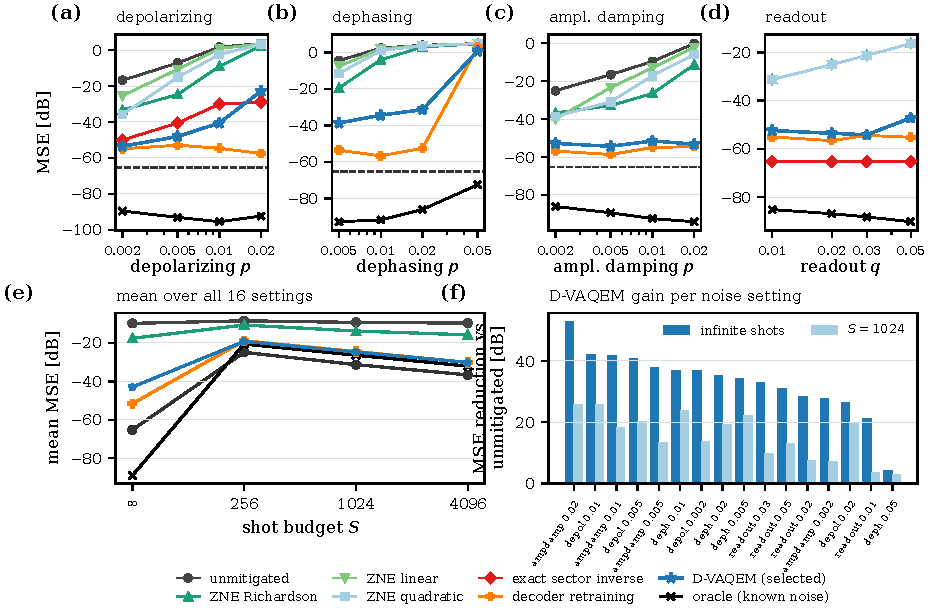
\includegraphics[width=\textwidth]{fig3_sweep.pdf}
\caption{\textbf{Headline comparison, $N=8$, infinite shots.}
\textbf{a--d}~Mean squared wrapped phase error versus noise strength for the
four channels; the dashed line is the noiseless decoder floor ($-65.3$ dB).
Zero-noise extrapolation is exactly blind to readout noise (panel \textbf{d}:
all ZNE curves coincide with the unmitigated one), while the learned map
inverts it and reaches the floor.
\textbf{e}~Mean over all sixteen settings versus shot budget, including the
noiseless floor and the known-noise-model oracle.
\textbf{f}~Per-setting MSE reduction of the holdout-selected \dvaqem{} variant
relative to the unmitigated estimator, at infinite shots and at $S=1024$.}
\label{fig:sweep}
\end{figure*}


Three comparisons isolate what the distribution-level formulation buys.
First, \dvaqem{} beats the best of the three ZNE variants in all sixteen
settings, by $25.0$ dB on average (minimum $4.0$ dB).  The gap has two distinct
origins.  For readout noise it is qualitative: unitary folding leaves a
readout channel invariant, so every ZNE variant returns \emph{exactly} the
unmitigated estimate (Table~\ref{tab:channels}, readout columns), whereas the
learned map inverts the flip kernel and reaches the noiseless floor
($-65.3$ dB, identical to the exact sector inverse).  For gate noise the gap is
quantitative and is explained by Proposition~\ref{prop:delta}: the
extrapolation coefficients amplify both the residual model error and, at
finite shots, the sampling noise.  Second, against noise-aware decoder
retraining---the strongest model-free baseline---\dvaqem{} is within $\sim1$ dB
at infinite shots (retraining wins $15/16$ settings there, as expected for a
baseline with $6$--$120\times$ more parameters and direct access to the
estimator objective) and is statistically indistinguishable at finite shots
(mean $-24.8$ dB versus $-24.5$ dB at $S=1024$), while using $81$--$1673$
instead of $9666$ trainable parameters, requiring no quantum--classical
re-optimisation loop, and leaving the certified decoder untouched.  Third, the
known-noise-model oracle remains far ahead (mean $-89.1$ dB at infinite shots,
a $46.1$ dB gap to \dvaqem{}): model-free mitigation is not free, and the gap
quantifies precisely what noise-model knowledge would buy.

At finite shots the picture changes in \dvaqem{}'s favour relative to the
floor: the mean gain over the unmitigated estimator is $10.7$, $15.4$ and
$20.5$ dB at $S=256,1024,4096$, and the residual distance to the
\emph{noiseless} shot-noise floor is only $5.7$, $6.6$ and $6.4$ dB, i.e.\
\dvaqem{} closes $65$--$76\,\%$ of the decibel gap that noise opens between the
unmitigated estimator and the ideal device (Fig.~\ref{fig:sweep}e,f).

Finally, the mitigated estimator uses the information present in the noisy
data essentially optimally: its mean squared error lies within $0.6$ dB of the
Cram\'er--Rao bound $1/(S F(\yvec))$ of the \emph{noisy} family at $S=1024$
($1.1$ dB at $S=4096$; range $-9.0$ to $+2.5$ dB over settings).  Points below
the bound are not a violation: the bound applies to unbiased estimators of the
noisy family, whereas the mitigated estimator trades a small residual bias
against variance, which is exactly what a bias--variance-aware mitigation
should do.

\subsection{Finite shots: validating and exploiting the delta method}
\label{subsec:shots}

Figure~\ref{fig:shots} tests Proposition~\ref{prop:delta} on three
representative settings over $S=64\dots8192$.  The analytic prediction
$\mathrm{bias}^2+\mathrm{Var}_S$ tracks the Monte-Carlo mean squared error over
$96$ (setting, method, $S$) points with a ratio in $[0.90,2.08]$, mean $1.03$,
median $1.00$; for the map-based estimators the ratio stays in
$[0.90,1.18]$, and the only deviations beyond $1.2$ are ZNE at $S\le256$,
where the extrapolated observable is far from Gaussian.  The closed-form
variance is therefore trustworthy both as an error bar and as a training
signal.

Exploiting it is worth a lot.  Refitting the shot-aware map at the operating
budget improves on the shot-independent cross-entropy map by up to $8.6$ dB
(depolarising), $12.8$ dB (amplitude damping) and $14.2$ dB (readout) at
$S=8192$, with the gain growing monotonically in $S$ as the bias term becomes
the limiting one (Fig.~\ref{fig:shots}d); at $S=64$ the two coincide, as they
must, because both are then variance-dominated.  The bias--variance
decomposition (Fig.~\ref{fig:shots}c) shows the mechanism: the shot-aware map
keeps the variance and reduces the squared bias by up to two orders of
magnitude.  A cold-start ablation (Table~\ref{tab:ablation}) shows that the
staged warm starts are a robustness device rather than a necessity in this
regime: refitting from scratch changes the deployed MSE by $-0.3$ dB on average
(worst case $+1.4$ dB) and changes the selected variant in $1/16$ settings.

\begin{figure*}[t]
\centering
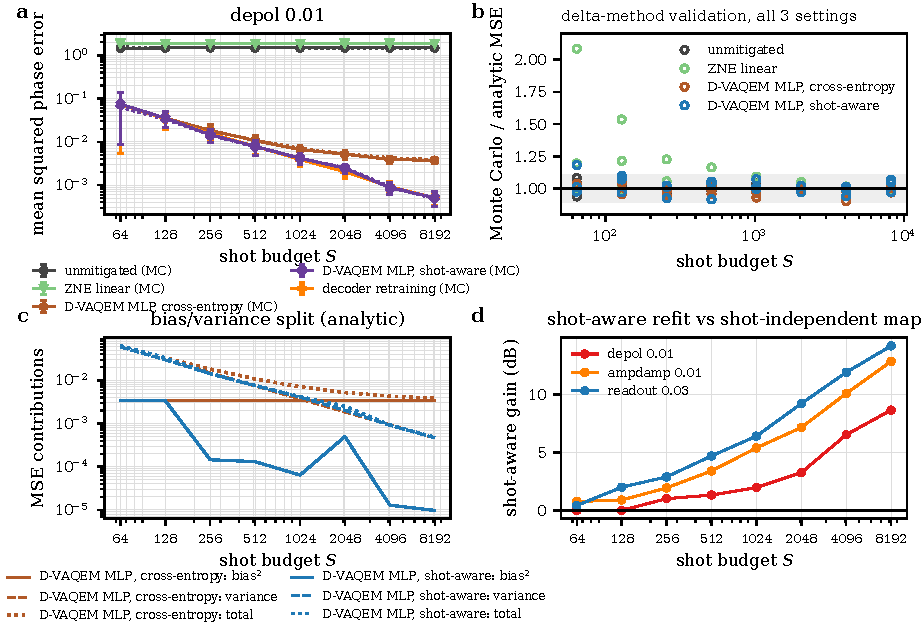
\includegraphics[width=\textwidth]{fig4_finite_shots.pdf}
\caption{\textbf{Finite shots and the delta method.}
\textbf{a}~Monte-Carlo mean squared error (markers, $41$ trials) and the
analytic prediction $\mathrm{bias}^2+\mathrm{Var}_S$ (dotted) versus shot
budget for depolarising $p=0.01$.
\textbf{b}~Ratio of Monte-Carlo to analytic MSE for all $96$ (setting, method,
$S$) points; the band marks $\pm10\,\%$.  The large deviations belong to ZNE at
$S\le256$.
\textbf{c}~Bias--variance decomposition of the shot-independent (cross-entropy)
and shot-aware maps: the shot-aware fit removes squared bias at no variance
cost.
\textbf{d}~Gain of refitting the map at the operating shot count, versus the
shot-independent map, for the three settings.}
\label{fig:shots}
\end{figure*}


\subsection{Scaling to ten qubits}
\label{subsec:scaling}

The scaling study repeats the full method suite at $N=4,6,8,10$ with
depolarising $p=0.01$ (Fig.~\ref{fig:scaling}, Table~\ref{tab:scaling}), each
size using its own independently trained interferometer.  The unmitigated
estimator degrades with $N$ (from $-5.8$ dB at $N=4$ to $+2.1$ dB at $N=10$ at
$S=1024$) because the same per-gate error rate acts on a larger probe; the
selected \dvaqem{} variant reduces the mean squared error by $30.1$, $44.2$,
$42.8$ and $34.7$ dB at infinite shots and by $19.2$, $23.6$, $25.9$ and
$18.3$ dB at $S=1024$, i.e.\ the mitigation does not decay with system size.
What changes with $N$ is the \emph{cost of the alternatives}: the calibration
data are $N+1=5\dots11$ numbers per phase and the linear map has
$(N+1)^2=25\dots121$ parameters, whereas a full-outcome map would need $4^N$
parameters ($1.05\times10^6$ at $N=10$) and process tomography of the probe
would need the same number of coefficients.  The measured wall-clock cost makes
the same point dynamically (Table~\ref{tab:cost}): fitting all seven
\dvaqem{} variants takes $21.6$--$22.8$ s at every $N$, the $21$-phase
calibration costs $0.01$--$48.5$ s of exact simulation, while the $361$-phase
oracle grid costs $0.1$ s at $N=4$ but $833$ s at $N=10$---and the underlying
exact dataset for the scaling study itself took $1981$ s at $N=10$.  At
$N=10$ the mitigated estimator ($-16.3$ dB at $S=1024$) still trails the
noiseless floor ($-25.9$ dB) by $\sim10$ dB, the largest residual in the study;
we attribute it to the combination of a strongly information-poor noisy family
($F(\yvec)/F(\tvec)=0.12$) and only $21$ calibration phases for an
$11$-dimensional distribution, and regard closing it as the main quantitative
target for hardware experiments.

\begin{figure*}[t]
\centering
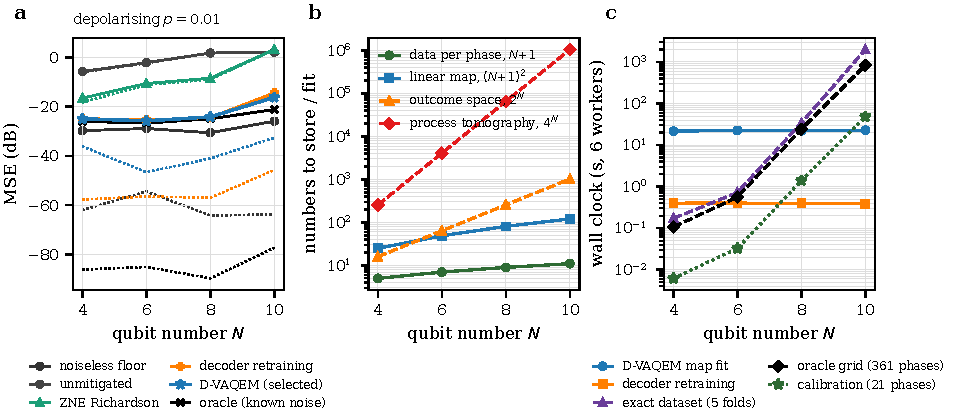
\includegraphics[width=\textwidth]{fig5_scaling.pdf}
\caption{\textbf{Scaling with qubit number} (depolarising $p=0.01$).
\textbf{a}~MSE versus $N$ at $S=1024$ (solid) and infinite shots (dotted) for
the method suite; each $N$ uses its own independently trained interferometer.
\textbf{b}~Data and parameter volumes: the sector formulation needs $N+1$
numbers per phase and $(N+1)^2$ map parameters, against $2^N$ outcomes and
$4^N$ process-tomography coefficients.
\textbf{c}~Measured wall-clock cost: the \dvaqem{} fit is flat in $N$
($\approx22$ s), the calibration grows linearly in the number of exact
simulations, and the $361$-phase known-noise-model oracle grid grows
exponentially ($833$ s at $N=10$).}
\label{fig:scaling}
\end{figure*}


\subsection{Calibration budget}
\label{subsec:calib}

Figure~\ref{fig:calib} asks how much calibration resource \dvaqem{} needs at
depolarising $p=0.01$, $S=1024$.  Along the phase axis, the linear shot-aware
map already delivers $-23.6$ dB (a $25.3$ dB reduction) from $n_{\rm cal}=5$
phases and saturates at $-24.2$ dB by $n_{\rm cal}=17$; the MLP maps need
$n_{\rm cal}\ge17$ to reach the same level, which is exactly the
sample-complexity price of their extra flexibility, and the holdout selection
correctly prefers the linear map when phases are scarce.  One point
($n_{\rm cal}=9$) is a visible selection failure---with only $7$ fitting phases
the holdout score picks an MLP variant, which gains $12.1$ dB instead of the
$\sim25$ dB the linear map delivers---and we report it as
the honest failure mode of data-driven selection at very small budgets.  Along
the precision axis, targets estimated from as few as $512$ shots per
calibration phase are as good as exact targets ($24.5$ versus $25.7$ dB
reduction), so the noiseless target may itself come from a modest device run
or from a classical model with sampling error.  Both axes confirm that the
resource consumed by \dvaqem{} is the standard VAQEM one---tens of calibrated
phase points---and not tomography.

\begin{figure*}[t]
\centering
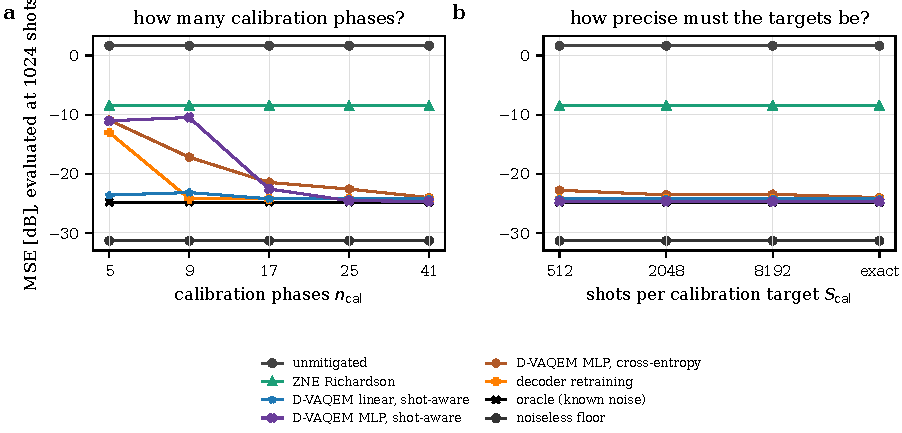
\includegraphics[width=\textwidth]{fig6_calibration.pdf}
\caption{\textbf{Calibration budget} (depolarising $p=0.01$, $N=8$, evaluated
at $S=1024$).
\textbf{a}~MSE versus the number of calibration phases: the linear shot-aware
map needs only five phases for a $25$ dB reduction; the MLP maps need
$\ge17$.  The point at $n_{\rm cal}=9$ is a holdout-selection failure, reported
as the failure mode of data-driven selection at tiny budgets.
\textbf{b}~MSE versus the number of shots used to estimate the calibration
targets: $512$ shots per phase are as good as exact targets.}
\label{fig:calib}
\end{figure*}


\subsection{Robustness: seeds, ablations and simulator validation}
\label{subsec:robust}

Repeating the entire headline sweep with three independent random seeds (map
initialisation, holdout sampling and Monte-Carlo trials) selects the identical
variant in all $16$ settings every time; the per-setting spread of the deployed
MSE is $0.00$ dB at infinite shots and at most $0.93$ dB (mean $0.46$ dB) at
$S=1024$, i.e.\ of the order of the Monte-Carlo error bar itself
(Table~\ref{tab:seeds}).  The cold-start ablation of
Sec.~\ref{subsec:shots} and the Fisher-weight choice ($\lambda=1$ throughout)
leave the conclusions unchanged.  Finally, every distribution used above comes
from a simulator that reproduces PennyLane's \texttt{default.mixed} to
$\le3.5\times10^{-13}$ and the stored VQ-CNNI checkpoints to machine precision,
and for which the sector reduction is verified information-preserving to
$2\times10^{-14}$ relative (Appendix~\ref{app:validation}), so the reported
gains are properties of the method and not of our numerical backend.

\section{Discussion}
\label{sec:discussion}

\paragraph{What the method assumes, and what it does not.}
\dvaqem{} assumes a stationary noise channel over the calibration window, a
classical model of the noiseless circuit (or a low-noise device that provides
the targets), and a decoder that is frozen after certification.  It assumes
\emph{nothing} about the channel itself: no tomography, no noise model, no
folded circuits at inference, and no modification of the certified estimator.
The price of model-freedom is visible in our numbers as the $46$ dB gap to the
known-noise-model oracle at infinite shots; where a trustworthy noise model
exists, the oracle (or probabilistic error cancellation built on it) remains
the better tool, and \dvaqem{} is the tool for the regime where no such model
is available---which is the regime of most near-term deployments.

\paragraph{Why distribution level, and why now.}
The sufficiency result (Theorem~\ref{thm:sufficiency}) is what turns
distribution-level mitigation from a heuristic into a complete description:
for collective probes the sector family is the estimation problem, so a map on
$N+1$ numbers loses nothing that a map on $2^N$ numbers could recover, while
its parameter count and calibration volume grow linearly instead of
exponentially.  This is complementary to, and compatible with, observable-level
VAQEM \cite{strikis2021learning,lowe2021unified}: whenever the readout of
interest is a linear observable, the two coincide; whenever the readout is a
learned nonlinear inverse---the situation in every neural quantum sensor
\cite{fiderer2021neural,gebhart2023learning,yang2025vqcnni}---only the
distribution-level object can be repaired without retraining the sensor.

\paragraph{Limitations.}
Our study is numerical: the noise is Markovian, gate-synchronous and stationary,
whereas hardware noise is correlated and drifting; extending the calibration
protocol to drifting channels (e.g.\ by interleaving recalibration phases) is
the natural next step.  The probe family is a single architecture (the
VQ-CNNI interferometer), although the sufficiency argument applies to any
probe whose readout is aggregated onto a collective statistic, and the four
independently trained checkpoints ($N=4,6,8,10$) already show that the
conclusions are not tied to one trained model.  The mitigated family is a
clipped quasi-probability, so its Fisher information is support-restricted and
must be read as a diagnostic (Fig.~\ref{fig:concept}c), not as a Cram\'er--Rao
bound; the largest clipped negative mass we observe is $0.10$.  And at
dephasing $p=0.05$ the noisy family retains $2\times10^{-4}$ of the clean
Fisher information: no mitigation, ours included, can create information that
the channel destroyed, and the honest statement there is that the sensor should
be re-designed rather than post-processed.

\section{Conclusion}
\label{sec:conclusion}

We have shown that error mitigation for learned quantum sensors is naturally
formulated at the level of measurement distributions, and that for
collective-spin probes this formulation is exact: the population imbalance is a
sufficient statistic for the phase, verified to machine precision and bounded
to $4.6\times10^{-3}$ dB of Cram\'er--Rao penalty under gate noise.  On this
$(N+1)$-dimensional space a small parametric map, trained on calibration data
alone and selected by a held-out calibration score, reduces the mean squared
phase error of an eight-qubit variational interferometer by $33.2$ dB at
infinite shots and closes $65$--$76\,\%$ of the decibel gap to the noiseless
device at $256$--$4096$ shots, beating zero-noise extrapolation in all sixteen
noise settings and matching noise-aware decoder retraining at finite shots with
two orders of magnitude fewer parameters.  A shot-aware objective built on the
exact delta-method variance makes the mitigation aware of the operating shot
budget and validates its own error bars analytically.  The approach scales to
ten qubits with eleven calibration numbers per phase, needs as few as five
calibration phases to buy $25$ dB, and operates within $0.6$ dB of the
Cram\'er--Rao bound of the noisy data.  Distribution-level mitigation is
therefore a practical, model-free route to deploying calibrated quantum sensors
on noisy hardware.

\begin{acknowledgments}
This work is partially supported by the National Key Research and Development
Program of China (NKRDC) under Grant No.~2021YFA0718803 and by the National
Natural Science Foundation of China (NSFC).  The authors thank the developers
of PennyLane and autograd, whose tools made the cross-validation in
Appendix~\ref{app:validation} possible.
\end{acknowledgments}

\bigskip\noindent
\textbf{Code and data availability}  All code (simulator, mitigation suite,
experiment drivers, figure and table generators) and all result files,
including the machine-readable digest of every number quoted here, are
archived with the manuscript source in the accompanying repository
\texttt{D-VAQEM} (\texttt{code/} for the simulator,
mitigation suite and drivers; \texttt{results/} for every
result file quoted here; \texttt{paper/} for the manuscript sources and the
generated tables).  The VQ-CNNI interferometer checkpoints and the
companion study are at \url{https://github.com/RichardYang88/VQ-CNNI}.

\appendix
\onecolumngrid

\section{Proofs}
\label{app:proofs}

\subsection{Delta-method variance of a mitigated estimate}
Write $\hat\yvec=\yvec+S^{-1/2}\bm\xi$ with
$\mathbb E[\bm\xi]=0$ and
$\mathrm{Cov}[\bm\xi]=\Sigma=\mathrm{diag}\,\yvec-\yvec\yvec^{\mathsf T}$, the
multinomial covariance.  A first-order Taylor expansion of the differentiable
readout $f$ gives
$\phihat=f(\yvec)+S^{-1/2}g^{\mathsf T}\bm\xi+o_p(S^{-1/2})$, hence
$\mathrm{Var}[\phihat]=S^{-1}g^{\mathsf T}\Sigma g+o(S^{-1})$, which is the
first claim.  For ZNE the estimator is
$\phihat=f(\sum_f c_f\hat\yvec_f)$ with \emph{independent} folds, so the
chain rule gives the gradient $c_f g_f$ with respect to fold $f$ and
$\mathrm{Var}[\phihat]=S^{-1}\sum_f c_f^2 g_f^{\mathsf T}\Sigma_f g_f$.  Since
$\Sigma_f\succeq0$ and $\sum_f c_f=1$ for any extrapolation that is exact at
zero noise, Cauchy--Schwarz gives $\sum_f c_f^2\ge1$, with equality only for
the trivial single-fold estimator: extrapolation necessarily amplifies shot
noise.  The values quoted in the main text, $\sum_f c_f^2=5.22$ (Richardson on
$(1,3,5)$), $1.46$ (linear fit) and $2.12$ (quadratic fit on $(1,3,5,7,9)$),
are read off the fitted coefficients stored with the results.

\subsection{Readout blindness of unitary folding}
\label{app:zne-blind}
Let the device noise be a readout channel $B$ acting on the sampled outcomes,
so that the measured family is $\yvec^{(f)}=B\,A\,p^{(f)}$ at fold $f$, where
$p^{(f)}$ is the ideal (noiseless) distribution of the folded circuit.  Unitary
folding satisfies $p^{(f)}=p^{(1)}$ for every odd $f$, because
$UU^\dagger=\mathbb 1$; hence $\yvec^{(f)}$ is independent of $f$ and any
extrapolation $\sum_f c_f \yvec^{(f)}$ with $\sum_f c_f=1$ returns exactly
$\yvec^{(1)}$, the unmitigated distribution.  This is why the ZNE columns for
readout noise in Table~\ref{tab:channels} coincide with the unmitigated row to
all printed digits.  The same argument shows that folding cannot mitigate any
channel that commutes with the folding operation, including measurement
assignment error, which is precisely the channel class that the learned
distribution-level map inverts.

\section{Simulator validation}
\label{app:validation}

All distributions in this work come from a NumPy/autograd Kraus
density-matrix simulator that applies an arbitrary single-qubit channel after
every gate and supports unitary folding.  It is validated by $53$ automated
checks (\texttt{code/validate\_simulator.py}), all of which pass:
(i) the noiseless statevector, real-representation and density-matrix paths
agree to $\le3\times10^{-15}$; (ii) trace preservation of every Kraus set and
normalisation of every output distribution; (iii) fold invariance of the
noiseless circuit ($\le6\times10^{-15}$); (iv) exactness of the sector
reduction, $A K_{\rm full}=K_m A$ for the noisy sector kernel, to
$1.1\times10^{-16}$, and information preservation
$F(\pvec_m)=F(\pvec_{\rm full})$ to $2.0\times10^{-14}$ relative;
(v) agreement with PennyLane~0.42 \texttt{default.mixed} at $N=4$ for
depolarising, dephasing, amplitude-damping and bit-flip channels and folds
$1,3,5$, with maximum deviation $3.5\times10^{-13}$ over outcome
probabilities, and agreement with the stored PennyLane-trained VQ-CNNI
checkpoints (median SWPE and SLD-QFI identical to all printed digits);
(vi) the flip-equivalent surrogate used only to accelerate the noiseless
calibration path deviates from the exact Kraus evolution by at most
$1.3\times10^{-2}$ in $p_m$ at the strongest depolarising rate considered, and
is never used in any reported evaluation.  The full check log ships with the
code.

\clearpage
% ============================ bibliography ============================
\bibliographystyle{apsrev4-2}
\bibliography{references}

\clearpage
% ============================ supplemental tables ========================
\setcounter{table}{0}
\renewcommand{\thetable}{S\arabic{table}}
\section*{Supplemental tables}
\label{app:supplement}
The tables below are generated directly from the result files by
\texttt{code/make\_tables.py}; the corresponding machine-readable digest is
\texttt{results/paper\_numbers.md} in the repository.
% auto-generated by code/make_tables.py -- do not edit
\begin{table*}[t]
\centering
\caption{MSE (dB) of every method in all 16 noise settings at infinite shots, $N=8$.  The last row is the variant selected by the held-out calibration score, which is the number reported in the main text.}
\label{tab:sweep_inf}
\tiny
\begin{tabular}{@{}lcccccccccccccccc@{}}
\hline
method & depol\ 0.002 & depol\ 0.005 & depol\ 0.01 & depol\ 0.02 & deph\ 0.005 & deph\ 0.01 & deph\ 0.02 & deph\ 0.05 & ampdamp\ 0.002 & ampdamp\ 0.005 & ampdamp\ 0.01 & ampdamp\ 0.02 & readout\ 0.01 & readout\ 0.02 & readout\ 0.03 & readout\ 0.05 \\
\hline
noiseless floor & -65.3 & -65.3 & -65.3 & -65.3 & -65.3 & -65.3 & -65.3 & -65.3 & -65.3 & -65.3 & -65.3 & -65.3 & -65.3 & -65.3 & -65.3 & -65.3 \\
unmitigated & -16.8 & -7.1 & 1.7 & 3.7 & -4.5 & 2.3 & 3.9 & 4.8 & -25.1 & -16.6 & -9.6 & -0.2 & -31.3 & -25.0 & -21.2 & -16.3 \\
ZNE, Richardson & -33.3 & -24.7 & -9.0 & 2.3 & -19.5 & -4.1 & 2.9 & 4.7 & -36.7 & -32.9 & -26.5 & -11.4 & -31.3 & -25.0 & -21.2 & -16.3 \\
ZNE, linear fit & -25.4 & -10.7 & 0.9 & 3.5 & -7.6 & 1.8 & 3.8 & 4.8 & -40.0 & -23.4 & -13.0 & -2.3 & -31.3 & -25.0 & -21.2 & -16.3 \\
ZNE, quadratic fit & -35.8 & -15.1 & -2.4 & 3.2 & -11.6 & 1.0 & 3.5 & 4.8 & -38.7 & -30.9 & -17.2 & -5.9 & -31.3 & -25.0 & -21.2 & -16.3 \\
exact sector inverse & -50.1 & -40.6 & -30.1 & -28.9 & -- & -- & -- & -- & -- & -- & -- & -- & -65.3 & -65.3 & -65.3 & -65.3 \\
decoder retraining & -54.9 & -52.9 & -54.6 & -57.6 & -53.6 & -56.7 & -52.5 & 2.9 & -56.9 & -58.7 & -55.0 & -54.5 & -55.0 & -56.6 & -54.4 & -55.2 \\
D-VAQEM linear, $\ell_2$ & -50.3 & -42.6 & -27.9 & -12.6 & -40.0 & -22.6 & -14.0 & 4.3 & -62.0 & -48.3 & -41.3 & -33.5 & -65.2 & -60.9 & -56.5 & -50.1 \\
D-VAQEM linear, CE & -50.3 & -42.6 & -9.8 & -18.7 & -40.0 & -13.7 & -15.3 & 3.8 & -62.0 & -48.3 & -41.3 & -16.6 & -29.3 & -31.5 & -26.5 & -30.4 \\
D-VAQEM linear, shot-aware & -53.5 & -41.4 & -40.6 & -22.8 & -38.7 & -34.4 & -20.0 & 1.0 & -52.8 & -54.4 & -51.5 & -42.4 & -52.4 & -53.5 & -54.1 & -53.8 \\
D-VAQEM MLP, $\ell_2$ & -27.1 & -26.7 & -21.3 & -27.8 & -25.2 & -26.3 & -26.2 & 0.1 & -24.3 & -22.6 & -24.8 & -25.2 & -22.5 & -23.5 & -24.3 & -26.5 \\
D-VAQEM MLP, CE & -27.1 & -26.7 & -24.7 & -26.8 & -25.2 & -27.0 & -21.8 & 0.7 & -24.3 & -23.9 & -24.1 & -23.1 & -23.0 & -24.1 & -24.3 & -23.8 \\
D-VAQEM MLP, CE+Fisher & -20.0 & -18.7 & -24.7 & -26.8 & -25.2 & -27.0 & -21.8 & 0.7 & -20.8 & -19.1 & -18.5 & -23.1 & -23.0 & -24.1 & -24.3 & -20.4 \\
D-VAQEM MLP, shot-aware & -50.3 & -48.1 & -48.9 & -32.9 & -47.0 & -34.0 & -31.4 & 0.1 & -47.9 & -32.2 & -47.7 & -53.2 & -48.0 & -48.7 & -48.8 & -47.2 \\
oracle, known noise (ML) & -89.6 & -93.1 & -95.5 & -92.4 & -92.8 & -91.8 & -86.1 & -72.5 & -86.1 & -89.4 & -92.5 & -94.1 & -85.2 & -86.9 & -88.2 & -90.2 \\
oracle, known noise ($\ell_2$) & -80.1 & -86.1 & -93.3 & -90.3 & -87.7 & -90.2 & -84.9 & -71.4 & -78.3 & -81.0 & -85.9 & -92.4 & -77.3 & -78.0 & -78.7 & -80.3 \\
D-VAQEM (selected) & -53.5 & -48.1 & -40.6 & -22.8 & -38.7 & -34.4 & -31.4 & 0.7 & -52.8 & -54.4 & -51.5 & -53.2 & -52.4 & -53.5 & -54.1 & -47.2 \\
\hline
\end{tabular}
\end{table*}


\begin{table*}[t]
\centering
\caption{MSE (dB) of every method in all 16 noise settings at $S=1024$, $N=8$.  The last row is the variant selected by the held-out calibration score, which is the number reported in the main text.}
\label{tab:sweep_S1024}
\tiny
\begin{tabular}{@{}lcccccccccccccccc@{}}
\hline
method & depol\ 0.002 & depol\ 0.005 & depol\ 0.01 & depol\ 0.02 & deph\ 0.005 & deph\ 0.01 & deph\ 0.02 & deph\ 0.05 & ampdamp\ 0.002 & ampdamp\ 0.005 & ampdamp\ 0.01 & ampdamp\ 0.02 & readout\ 0.01 & readout\ 0.02 & readout\ 0.03 & readout\ 0.05 \\
\hline
noiseless floor & -31.3 & -31.3 & -31.3 & -31.3 & -31.3 & -31.3 & -31.3 & -31.3 & -31.3 & -31.3 & -31.3 & -31.3 & -31.3 & -31.3 & -31.3 & -31.3 \\
unmitigated & -16.5 & -7.0 & 1.7 & 3.7 & -4.3 & 2.4 & 3.9 & 4.8 & -23.8 & -16.4 & -9.6 & -0.2 & -27.8 & -23.7 & -20.4 & -16.1 \\
ZNE, Richardson & -23.6 & -20.8 & -8.5 & 2.4 & -17.7 & -3.5 & 2.9 & 4.7 & -24.0 & -23.4 & -21.6 & -11.1 & -22.4 & -20.6 & -18.3 & -15.1 \\
ZNE, linear fit & -23.2 & -10.6 & 0.9 & 3.5 & -7.6 & 1.8 & 3.8 & 4.8 & -29.0 & -22.3 & -12.8 & -2.1 & -26.6 & -23.3 & -20.3 & -15.9 \\
ZNE, quadratic fit & -26.5 & -14.9 & -2.2 & 3.2 & -11.3 & 1.0 & 3.5 & 4.8 & -26.6 & -25.9 & -16.6 & -5.8 & -25.9 & -22.6 & -20.1 & -15.8 \\
exact sector inverse & -29.4 & -24.1 & -3.9 & 3.7 & -- & -- & -- & -- & -- & -- & -- & -- & -30.5 & -30.3 & -29.7 & -29.0 \\
decoder retraining & -29.3 & -27.2 & -24.2 & -17.8 & -27.1 & -22.5 & -14.2 & 3.1 & -29.9 & -29.3 & -28.1 & -26.4 & -30.4 & -30.1 & -29.6 & -28.8 \\
D-VAQEM linear, $\ell_2$ & -29.2 & -25.4 & -18.8 & -10.1 & -23.5 & -16.5 & -6.0 & 4.2 & -29.9 & -29.1 & -26.4 & -20.1 & -30.5 & -30.2 & -29.5 & -28.7 \\
D-VAQEM linear, CE & -29.2 & -25.4 & -9.1 & -14.1 & -23.5 & -12.6 & -9.5 & 3.9 & -29.9 & -29.1 & -26.4 & -15.5 & -26.3 & -27.0 & -24.5 & -25.5 \\
D-VAQEM linear, shot-aware & -30.1 & -27.0 & -24.1 & -16.0 & -26.6 & -21.6 & -12.7 & 2.9 & -30.8 & -29.9 & -28.0 & -25.7 & -31.4 & -31.2 & -30.3 & -29.2 \\
D-VAQEM MLP, $\ell_2$ & -25.4 & -23.9 & -20.0 & -17.8 & -23.3 & -21.4 & -14.5 & 1.9 & -23.5 & -22.0 & -23.0 & -22.4 & -22.0 & -23.0 & -23.5 & -24.6 \\
D-VAQEM MLP, CE & -25.4 & -23.9 & -22.0 & -17.0 & -23.3 & -20.9 & -13.8 & 2.0 & -23.5 & -23.0 & -22.8 & -21.6 & -22.6 & -23.4 & -23.5 & -22.8 \\
D-VAQEM MLP, CE+Fisher & -19.6 & -18.1 & -22.0 & -17.0 & -23.3 & -20.9 & -13.8 & 2.0 & -20.3 & -18.8 & -18.0 & -21.6 & -22.6 & -23.4 & -23.5 & -19.8 \\
D-VAQEM MLP, shot-aware & -30.1 & -27.3 & -24.5 & -18.2 & -27.5 & -22.6 & -15.5 & 1.9 & -30.6 & -28.6 & -28.5 & -26.0 & -30.9 & -30.8 & -30.1 & -29.1 \\
oracle, known noise (ML) & -32.0 & -28.2 & -24.8 & -18.4 & -28.1 & -23.2 & -15.5 & 2.7 & -34.2 & -31.7 & -29.4 & -27.2 & -34.5 & -33.8 & -32.8 & -31.2 \\
oracle, known noise ($\ell_2$) & -31.1 & -27.6 & -24.0 & -17.3 & -27.0 & -22.6 & -14.4 & 3.0 & -33.3 & -31.1 & -28.6 & -26.4 & -33.7 & -33.2 & -32.1 & -30.3 \\
D-VAQEM (selected) & -30.1 & -27.3 & -24.1 & -16.0 & -26.6 & -21.6 & -15.5 & 2.0 & -30.8 & -29.9 & -28.0 & -26.0 & -31.4 & -31.2 & -30.3 & -29.1 \\
\hline
\end{tabular}
\end{table*}


\begin{table*}[t]
\centering
\caption{Sufficiency of the collective-imbalance reduction: classical Fisher information of the full outcome distribution and of the sector distribution, Cramér--Rao penalty of the reduction, and worst pointwise relative deviation, for trained and random circuit parameters.}
\label{tab:e1}
\tiny
\begin{tabular}{@{}ccclrrr@{}}
\hline
$N$ & variant & noise & mean $F(\mathbf{p}_{\rm full})$ & mean $F(\mathbf{p}_m)$ & $\Delta_{\rm CRB}$ (dB) & max rel. dev. \\
\hline
4 & trained & noiseless & 1.328385 & 1.328385 & 0.00e+00 & 4.89e-16 \\
4 & trained & depol\_0.002 & 0.917365 & 0.917354 & 4.77e-05 & 2.32e-05 \\
4 & trained & depol\_0.01 & 0.391666 & 0.391637 & 3.21e-04 & 1.67e-04 \\
4 & trained & depol\_0.02 & 0.188023 & 0.187999 & 5.57e-04 & 5.81e-04 \\
4 & trained & readout\_0.03 & 0.914439 & 0.914439 & 0.00e+00 & 5.13e-16 \\
4 & random & noiseless & 1.679375 & 1.679375 & 0.00e+00 & 5.71e-16 \\
4 & random & depol\_0.002 & 1.315303 & 1.315300 & 8.02e-06 & 1.86e-05 \\
4 & random & depol\_0.01 & 0.721011 & 0.720998 & 7.89e-05 & 4.07e-04 \\
4 & random & depol\_0.02 & 0.379560 & 0.379544 & 1.84e-04 & 3.05e-03 \\
4 & random & readout\_0.03 & 1.319053 & 1.319053 & 6.66e-16 & 5.20e-16 \\
6 & trained & noiseless & 2.963040 & 2.963040 & 0.00e+00 & 3.56e-16 \\
6 & trained & depol\_0.002 & 1.546289 & 1.546274 & 4.12e-05 & 1.36e-05 \\
6 & trained & depol\_0.01 & 0.497582 & 0.497544 & 3.31e-04 & 1.55e-04 \\
6 & trained & depol\_0.02 & 0.192873 & 0.192846 & 6.12e-04 & 6.31e-04 \\
6 & trained & readout\_0.03 & 1.654670 & 1.654670 & 0.00e+00 & 6.12e-16 \\
6 & random & noiseless & 2.407917 & 2.407917 & 0.00e+00 & 5.14e-16 \\
6 & random & depol\_0.002 & 0.996009 & 0.995966 & 1.85e-04 & 2.07e-04 \\
6 & random & depol\_0.01 & 0.487688 & 0.487486 & 1.80e-03 & 1.25e-02 \\
6 & random & depol\_0.02 & 0.225289 & 0.225137 & 2.93e-03 & 6.00e-03 \\
6 & random & readout\_0.03 & 1.100621 & 1.100621 & 0.00e+00 & 4.05e-16 \\
8 & trained & noiseless & 5.022948 & 5.022948 & -8.88e-16 & 1.79e-15 \\
8 & trained & depol\_0.002 & 1.744551 & 1.744395 & 3.88e-04 & 2.17e-04 \\
8 & trained & depol\_0.01 & 0.303947 & 0.303854 & 1.34e-03 & 5.86e-04 \\
8 & trained & depol\_0.02 & 0.077225 & 0.077196 & 1.65e-03 & 6.99e-04 \\
8 & trained & readout\_0.03 & 2.281819 & 2.281819 & -1.33e-15 & 2.52e-15 \\
8 & random & noiseless & 3.736410 & 3.736410 & -2.66e-15 & 6.82e-16 \\
8 & random & depol\_0.002 & 2.242953 & 2.242749 & 3.95e-04 & 4.19e-04 \\
8 & random & depol\_0.01 & 0.737152 & 0.736962 & 1.12e-03 & 1.88e-03 \\
8 & random & depol\_0.02 & 0.196287 & 0.196077 & 4.65e-03 & 5.80e-03 \\
8 & random & readout\_0.03 & 2.847747 & 2.847747 & 0.00e+00 & 1.42e-15 \\
10 & trained & noiseless & 2.024544 & 2.024544 & 0.00e+00 & 3.02e-15 \\
10 & trained & depol\_0.002 & 0.466597 & 0.466549 & 4.51e-04 & 2.72e-04 \\
10 & trained & depol\_0.01 & 0.231981 & 0.231940 & 7.67e-04 & 1.92e-03 \\
10 & trained & depol\_0.02 & 0.105510 & 0.105495 & 6.51e-04 & 3.56e-03 \\
10 & trained & readout\_0.03 & 0.705204 & 0.705204 & 6.66e-16 & 3.06e-15 \\
10 & random & noiseless & 7.957316 & 7.957316 & 3.55e-15 & 7.42e-15 \\
10 & random & depol\_0.002 & 2.710680 & 2.710407 & 4.38e-04 & 3.52e-04 \\
10 & random & depol\_0.01 & 0.598831 & 0.598686 & 1.05e-03 & 1.79e-03 \\
10 & random & depol\_0.02 & 0.180223 & 0.180187 & 8.46e-04 & 4.75e-03 \\
10 & random & readout\_0.03 & 3.989421 & 3.989421 & 1.78e-15 & 5.72e-15 \\
\hline
\end{tabular}
\end{table*}


\begin{table*}[t]
\centering
\caption{Monte-Carlo mean squared phase error versus shot budget for the three settings of the finite-shot study (41 trials per point).}
\label{tab:e3mc}
\tiny
\begin{tabular}{@{}llcccccccc@{}}
\hline
setting & method & $S64$ & $S128$ & $S256$ & $S512$ & $S1024$ & $S2048$ & $S4096$ & $S8192$ \\
\hline
depol\_0.01 & unmitigated & 1.46e+00 & 1.48e+00 & 1.49e+00 & 1.48e+00 & 1.48e+00 & 1.48e+00 & 1.48e+00 & 1.48e+00 \\
depol\_0.01 & D-VAQEM MLP, CE & 7.41e-02 & 3.54e-02 & 1.83e-02 & 1.07e-02 & 6.59e-03 & 5.17e-03 & 3.88e-03 & 3.72e-03 \\
depol\_0.01 & D-VAQEM MLP, shot-aware & 7.41e-02 & 3.54e-02 & 1.45e-02 & 7.88e-03 & 4.19e-03 & 2.44e-03 & 8.66e-04 & 5.08e-04 \\
depol\_0.01 & decoder retraining & 7.28e-02 & 3.43e-02 & 1.55e-02 & 7.87e-03 & 3.91e-03 & 2.02e-03 & 9.12e-04 & 5.06e-04 \\
depol\_0.01 & ZNE, linear fit & 1.90e+00 & 1.88e+00 & 1.88e+00 & 1.88e+00 & 1.89e+00 & 1.90e+00 & 1.89e+00 & 1.89e+00 \\
ampdamp\_0.01 & unmitigated & 1.74e-01 & 1.35e-01 & 1.23e-01 & 1.14e-01 & 1.10e-01 & 1.10e-01 & 1.10e-01 & 1.09e-01 \\
ampdamp\_0.01 & D-VAQEM MLP, CE & 3.00e-02 & 1.71e-02 & 9.93e-03 & 7.16e-03 & 5.29e-03 & 4.64e-03 & 4.22e-03 & 4.16e-03 \\
ampdamp\_0.01 & D-VAQEM MLP, shot-aware & 2.51e-02 & 1.39e-02 & 6.35e-03 & 3.27e-03 & 1.53e-03 & 8.95e-04 & 4.15e-04 & 2.17e-04 \\
ampdamp\_0.01 & decoder retraining & 2.75e-02 & 1.39e-02 & 6.83e-03 & 3.38e-03 & 1.70e-03 & 8.12e-04 & 4.18e-04 & 2.01e-04 \\
ampdamp\_0.01 & ZNE, linear fit & 3.00e-01 & 2.87e-01 & 2.42e-01 & 2.29e-01 & 2.25e-01 & 2.22e-01 & 2.21e-01 & 2.23e-01 \\
readout\_0.03 & unmitigated & 2.92e-02 & 1.82e-02 & 1.22e-02 & 9.90e-03 & 9.16e-03 & 8.10e-03 & 7.79e-03 & 7.68e-03 \\
readout\_0.03 & D-VAQEM MLP, CE & 1.73e-02 & 9.94e-03 & 6.67e-03 & 5.17e-03 & 4.51e-03 & 4.18e-03 & 3.93e-03 & 3.83e-03 \\
readout\_0.03 & D-VAQEM MLP, shot-aware & 1.57e-02 & 6.27e-03 & 3.43e-03 & 1.75e-03 & 1.03e-03 & 5.02e-04 & 2.54e-04 & 1.47e-04 \\
readout\_0.03 & decoder retraining & 1.78e-02 & 9.11e-03 & 4.07e-03 & 2.06e-03 & 1.21e-03 & 5.67e-04 & 2.77e-04 & 1.49e-04 \\
readout\_0.03 & ZNE, linear fit & 2.81e-02 & 1.61e-02 & 1.10e-02 & 9.62e-03 & 8.62e-03 & 8.09e-03 & 7.74e-03 & 7.67e-03 \\
\hline
\end{tabular}
\end{table*}

\begin{table*}[t]
\centering
\caption{Ratio of the Monte-Carlo MSE to the analytic (delta-method) prediction bias$^2$ + Var$_S$.  A value of 1 validates the closed-form variance that the shot-aware objective minimises.}
\label{tab:e3ratio}
\tiny
\begin{tabular}{@{}llcccccccc@{}}
\hline
setting & method & $S64$ & $S128$ & $S256$ & $S512$ & $S1024$ & $S2048$ & $S4096$ & $S8192$ \\
\hline
depol\_0.01 & unmitigated & 0.940 & 0.977 & 0.995 & 0.992 & 0.995 & 1.000 & 1.000 & 0.999 \\
depol\_0.01 & D-VAQEM MLP, CE & 1.182 & 1.072 & 1.007 & 0.990 & 0.932 & 0.990 & 0.904 & 0.970 \\
depol\_0.01 & D-VAQEM MLP, shot-aware & 1.182 & 1.072 & 1.012 & 1.035 & 1.012 & 0.973 & 0.941 & 1.068 \\
depol\_0.01 & ZNE, linear fit & 1.002 & 0.993 & 0.994 & 0.994 & 0.999 & 1.004 & 1.001 & 0.999 \\
ampdamp\_0.01 & unmitigated & 1.082 & 1.005 & 1.012 & 0.989 & 0.983 & 0.995 & 1.003 & 1.003 \\
ampdamp\_0.01 & D-VAQEM MLP, CE & 1.038 & 1.044 & 0.979 & 1.020 & 0.969 & 0.991 & 0.984 & 1.016 \\
ampdamp\_0.01 & D-VAQEM MLP, shot-aware & 1.012 & 1.100 & 1.024 & 1.054 & 0.998 & 1.020 & 1.015 & 0.972 \\
ampdamp\_0.01 & ZNE, linear fit & 1.195 & 1.215 & 1.057 & 1.018 & 1.009 & 0.997 & 0.994 & 1.004 \\
readout\_0.03 & unmitigated & 1.044 & 1.025 & 0.969 & 0.982 & 1.042 & 0.993 & 0.994 & 1.000 \\
readout\_0.03 & D-VAQEM MLP, CE & 1.015 & 0.957 & 0.947 & 0.961 & 0.992 & 1.012 & 1.000 & 1.003 \\
readout\_0.03 & D-VAQEM MLP, shot-aware & 0.978 & 0.972 & 0.927 & 0.918 & 1.073 & 1.023 & 0.993 & 1.047 \\
readout\_0.03 & ZNE, linear fit & 2.083 & 1.535 & 1.227 & 1.165 & 1.093 & 1.051 & 1.017 & 1.015 \\
\hline
\end{tabular}
\end{table*}


\begin{table}[t]
\centering
\caption{MSE (dB) at $S=1024$ versus calibration phases $n_{\rm cal}$ (depolarising $p=0.01$, $N=8$).}
\label{tab:e5_n_cal}
\scriptsize
\begin{tabular}{@{}lccccc@{}}
\hline
method & 5 & 9 & 17 & 25 & 41 \\
\hline
unmitigated & 1.7 & 1.7 & 1.7 & 1.7 & 1.7 \\
ZNE, Richardson & -8.5 & -8.5 & -8.5 & -8.5 & -8.5 \\
D-VAQEM linear, shot-aware & -23.6 & -23.2 & -24.2 & -24.2 & -24.2 \\
D-VAQEM MLP, CE & -10.9 & -17.2 & -21.4 & -22.6 & -24.0 \\
D-VAQEM MLP, shot-aware & -11.0 & -10.5 & -22.6 & -24.5 & -24.6 \\
decoder retraining & -13.0 & -24.2 & -24.2 & -24.2 & -24.2 \\
oracle, known noise (ML) & -24.8 & -24.8 & -24.8 & -24.8 & -24.8 \\
noiseless floor & -31.3 & -31.3 & -31.3 & -31.3 & -31.3 \\
\hline
\end{tabular}
\end{table}

\begin{table}[t]
\centering
\caption{MSE (dB) at $S=1024$ versus calibration shots $S_{\rm cal}$ (depolarising $p=0.01$, $N=8$).}
\label{tab:e5_cal_shots}
\scriptsize
\begin{tabular}{@{}lcccc@{}}
\hline
method & 512 & 2048 & 8192 & exact \\
\hline
unmitigated & 1.7 & 1.7 & 1.7 & 1.7 \\
ZNE, Richardson & -8.5 & -8.5 & -8.5 & -8.5 \\
D-VAQEM linear, shot-aware & -24.2 & -24.2 & -24.2 & -24.2 \\
D-VAQEM MLP, CE & -22.8 & -23.6 & -23.5 & -24.0 \\
D-VAQEM MLP, shot-aware & -24.6 & -24.6 & -24.6 & -24.6 \\
decoder retraining & -24.2 & -24.2 & -24.2 & -24.2 \\
oracle, known noise (ML) & -24.8 & -24.8 & -24.8 & -24.8 \\
noiseless floor & -31.3 & -31.3 & -31.3 & -31.3 \\
\hline
\end{tabular}
\end{table}



\begin{table}[t]
\centering
\caption{Repeat runs of the headline sweep with independent random seeds: mean MSE reduction over the 16 settings and the set of selected variants.}
\label{tab:seeds}
\scriptsize
\begin{tabular}{@{}lccc@{}}
\hline
run & gain (dB) $\infty$ & gain (dB) $S1024$ & selected variants \\
\hline
seed0 & 33.16 & 15.42 & lin\_mse, mlp\_fisher, mlp\_mse \\
seed1 & 33.16 & 15.38 & lin\_mse, mlp\_fisher, mlp\_mse \\
seed2 & 33.16 & 15.42 & lin\_mse, mlp\_fisher, mlp\_mse \\
\hline
\end{tabular}
\end{table}

\begin{table*}[t]
\centering
\caption{Ablation of the staged warm start: the shot-aware maps are fitted from a cold start instead of being refined from the $\ell_2$/CE fits, and the held-out score re-selects the variant.}
\label{tab:ablation}
\tiny
\begin{tabular}{@{}lccccc@{}}
\hline
setting & warm variant & cold variant & warm (dB) & cold (dB) & cold$-$warm \\
\hline
ampdamp\_0.002 & lin\_mse & lin\_mse & -52.8 & -52.8 & +0.0 \\
ampdamp\_0.005 & lin\_mse & lin\_mse & -54.4 & -54.4 & +0.0 \\
ampdamp\_0.01 & lin\_mse & lin\_mse & -51.5 & -50.1 & +1.4 \\
ampdamp\_0.02 & mlp\_mse & mlp\_mse & -53.2 & -53.2 & +0.0 \\
deph\_0.005 & lin\_mse & lin\_mse & -38.7 & -38.7 & +0.0 \\
deph\_0.01 & lin\_mse & lin\_mse & -34.4 & -34.4 & +0.0 \\
deph\_0.02 & mlp\_mse & mlp\_mse & -31.4 & -31.4 & +0.0 \\
deph\_0.05 & mlp\_fisher & mlp\_fisher & 0.7 & 0.7 & +0.0 \\
depol\_0.002 & lin\_mse & lin\_mse & -53.5 & -55.2 & -1.7 \\
depol\_0.005 & mlp\_mse & mlp\_mse & -48.1 & -48.1 & +0.0 \\
depol\_0.01 & lin\_mse & lin\_mse & -40.6 & -40.6 & +0.0 \\
depol\_0.02 & lin\_mse & mlp\_fisher & -22.8 & -26.8 & -4.0 \\
readout\_0.01 & lin\_mse & lin\_mse & -52.4 & -52.4 & +0.0 \\
readout\_0.02 & lin\_mse & lin\_mse & -53.5 & -53.5 & +0.0 \\
readout\_0.03 & lin\_mse & lin\_mse & -54.1 & -54.1 & +0.0 \\
readout\_0.05 & mlp\_mse & mlp\_mse & -47.2 & -47.2 & +0.0 \\
\hline
\end{tabular}
\end{table*}



\end{document}
